\documentclass[utf8]{article}

%\usepackage{doi}
\usepackage{authblk}
\usepackage[T1]{fontenc}
\usepackage[utf8]{inputenc}
\usepackage[pdftex]{xcolor}
\usepackage[pdftex]{graphicx}
\usepackage[authoryear,round]{natbib}

% review mode
\usepackage{geometry}
\usepackage{lineno}
\linenumbers
\linespread{1.5}

% custom colours
\definecolor{darkblue}{cmyk}{0.9,0.3,0.0,0.0}
\definecolor{darkgreen}{cmyk}{0.8,0.0,1.0,0.0}
\definecolor{darkred}{cmyk}{0.1,0.9,0.8,0.0}
\definecolor{darkorange}{cmyk}{0.0,0.5,1.0,0.0}
\definecolor{darkpurple}{cmyk}{0.6,0.7,0.0,0.0}
\definecolor{darkbrown}{cmyk}{0.23,0.73,0.98,0.12}

% custom commands
\newcommand{\idea}[1]{\textcolor{darkgreen}{\emph{[\textbf{IDEA:} #1]}}}
\newcommand{\note}[1]{\textcolor{darkblue}{\emph{[\textbf{NOTE:} #1]}}}
\newcommand{\todo}[1]{\textcolor{darkred}{\emph{[\textbf{TODO:} #1]}}}
\newcommand{\aref}[0]{\textcolor{darkblue}{\textbf{[REF.]}}}
\newcommand{\ian}[1]{\textcolor{darkbrown}{\emph{[\textbf{IAN:} #1]}}}

\graphicspath{{../../figures/}}

\title{Last glacial cycle glacier erosion potential in the Alps}
\author[1]{Julien Seguinot}
\author[2]{Ian Delaney}
\affil[1]{Anafi, Greece} % {\small (juseg \emph{at} posteo.eu)}}
\affil[2]{Institute of Earth Surface Dynamics, University of Lausanne, Switzerland}


% ======================================================================
\begin{document}
% ======================================================================

\maketitle

\begin{abstract}

    The glacial landscape of the Alps has fascinated generations of explorers,
    artists, mountaineers and scientists with its diversity, including
    erosional features of all scales from high-mountain cirques, to steep
    glacial valleys and large over-deepened basins. Using previous glacier
    modelling results, and empirical inferences bedrock erosion under modern
    glaciers, we compute a distribution of potential glacier erosion in the Alps
    over the last glacial cycle from 120\,000 years ago to the present.
    %
    Despite large uncertainties related to the climate history of the Alps and
    unconstrained glacier erosion processes, the resulting modelled patterns of
    glacier erosion shows persistent features. The cumulative imprint of
    the last glacial cycle shows a very strong localization of glacier erosion
    with local maxima at the mouths of major Alpine valleys and some other
    upstream sections where glaciers are modelled to have flown with the
    highest velocity. The modelled erosion rates vary significantly through the
    glacial cycle, but show paradoxically little relation to the glaciation
    extent. Phases of glacier advance and maximum extension, characterized by
    low air and glacier temperatures, see a localization of rapid erosion rates
    at low elevation, while intra-montane areas are modelled to date from phases
    of intermediate glacier cover. The modelled erosion rates peak during
    deglaciation phases, when higher air and glacier temperature enhance
    glacier dynamics.
    %
    Our results depict the Alpine glacier erosion landscape as a
    time-transgressive patchwork, with different erosional landscapes of the
    same mountain range corresponding to different glaciation stages and time
    periods, thus offering insight into its diversity.

\end{abstract}


% ----------------------------------------------------------------------
\section{Introduction}
% ----------------------------------------------------------------------

    The glacial erosion landscape of the Alps has fascinated generations of
    explorers, artists, mountaineers and scientists for centuries. Its cultural
    impact is indeed so far-reaching, that in English, a non-Alpine language,
    the adjective ``alpine'' with non-capital ``a'' is now casually used to
    describe an Alpine-like, glacially modified mountain landscape outside the
    Alps, while the proper noun ``Alps'' has been applied to nick-name
    Alpine-like, glacier eroded mountain ranges in Norway (\emph{Lyngsalpene}),
    New Zealand (Southern Alps), Japan (\emph{Nihon Arupusu}), and elsewhere.

    Some mountain ranges are predominantly characterised by cirque glaciation
    (e.g. Uinta Mountains), glacial valleys (e.g. Putorana Plateau), or
    large-scale overdeepenings (e.g. Patagonia). But other regions, including
    the Alps, present a higher variety glacial erosional landforms
    (Fig.~\ref{fig:landscape}), whose implications on glacial history is yet to
    be understood.

    In absence of other glacial landforms, the degree of glacial modification
    of a landscape has sometimes been used as a proxy for the duration of past
    glacier cover, as for instance in geomorphological mapping \aref. However,
    cold-based glaciers have been shown to preserve landforms as fragile as
    sand beaches \aref. Yet it remains unclear how sharp the erosional
    transition to cold-based ice is, and why some glaciated regions show
    glacially preserved landscapes and others, including the Alps, do not
    \aref.

    While it has long been understood that glaciers leave a specific erosional
    imprint on the landscape, observing and quantifying the long-term erosion
    and sedimentation processes has been a challenge, not least due to the
    inaccessibility of glacier beds and the slow and stochastic nature of
    glacial erosion processes \aref. \ian{Perhaps this needs more detail?}

    More recent studies have moved away from process
    understanding towards attempts at calibrating empirical erosion laws for an entire
    glacier or set of glaciers. \citet{Koppes.etal.2015} quantified sediment
    yields in 15~Patagonian and Antarctic Peninsula fjords, concluding at a
    predominant control of surface air temperature on rapid glacier erosion and
    calibrating a near-square-law from glacier velocity to erosion rate.
    \citet{Herman.etal.2015} collected suspended sediment samples for 5~months
    in the outlet stream of Franz-Josef Glacier, mapped their chemical
    composition to geologic zones of distinctive glacier speed, and also
    concluded to a near-square relationship between basal sliding and glacier
    erosion, but yielding much higher erosion rates.
    \citet{Cook.etal.2020} assembled a global compilation of erosion rates for
    38~glaciers, showing a predominant role of glacier sliding velocity over
    climate variables, yet concluding at a sub-linear relationship to erosion.

    Here, the non-linear erosion law by \citet{Koppes.etal.2015} is applied to
    previously published model results \citep{Seguinot.etal.2018} and the
    patterns of modelled erosion rate and cumulative last glacial cycle erosion
    potential are analysed. Despite aggregated uncertainties on paleoclimate,
    glacier flow and glacier erosion processes, out results provide insights
    into the diversity of the Alpine glacial erosion landscape.


% ----------------------------------------------------------------------
\section{Methods}
% ----------------------------------------------------------------------

% -- -- -- -- -- -- -- -- -- -- -- -- -- -- -- -- -- -- -- -- -- -- -- -
\subsection{Ice sheet modelling}
% -- -- -- -- -- -- -- -- -- -- -- -- -- -- -- -- -- -- -- -- -- -- -- -

    The ice-sheet model set-up was presented in an earlier publication
    \citep{Seguinot.etal.2018} and is briefly summarized here. The simulations
    were conducted using the Parallel Ice Sheet Model (PISM, development
    version~e9d2d1f), an open-source, finite-difference, shallow-ice and
    shallow-shelf model
    \citep{PISM-authors.2017}. The model includes temperature and water-content
    dependent creep, pseudo-plastic basal sliding accounting for till
    dilatation under high water pressure, bedrock deformation under the ice
    load, and a~positive degree-day (PDD) surface mass balance model. The model
    is initialized with assumed present-day ice thickness and equilibrium
    ice and bedrock temperature at 120\,ka, and ran to the present.
    The ice-sheet model physical parameters are listed in the earlier
    open-access publication \citep{Seguinot.etal.2018}, and the complete PISM
    set-up is stored in long-term archived model output metadata for the
    present study \todo{upload}, and for the earlier publication
    \citep{Seguinot.2020, Seguinot.2020a}.

    Climate forcing is provided by a~monthly climatology from interpolated
    observational data \citep[WorldClim;][]{Hijmans.etal.2005} and the European
    Centre for Medium-Range Weather Forecasts Reanalysis Interim
    \citep[ERA-Interim;][]{Dee.etal.2011}, amended with temperature lapse-rate
    corrections from the European Project for Ice Coring in Antarctica
    \citep[EPICA;][] {Jouzel.etal.2007}, and time-dependent paleo-precipitation
    reductions \citep{Huybrechts.2002}. Lower-resolution runs based on
    alternative paleoclimate scenarios \citep{Seguinot.etal.2018} are analyzed
    in the discussion part (Sect.~\ref{sec:sensitivity}).

% -- -- -- -- -- -- -- -- -- -- -- -- -- -- -- -- -- -- -- -- -- -- -- -
\subsection{Erosion law}
% -- -- -- -- -- -- -- -- -- -- -- -- -- -- -- -- -- -- -- -- -- -- -- -

    Modelled erosion rates, $\dot{e}$, are calculated from the modelled basal
    velocities, $u_\mathrm{b}$, using a empirical erosion power-law,
    %
    \begin{equation}
        \dot{e} = K_\mathrm{g} u_\mathrm{b}^l ,
    \end{equation}
    %
    where $K_g = 5.2\times 10^{-11}\,m^{1-l}\,a^{l-1}$ and $l = 2.34$ are
    empirical constants calibrated on quantified fjord sediment yields and
    velocities from 15~Patagonian and Antarctic Peninsula tidewater glaciers
    \citep{Koppes.etal.2015}. Alternative erosion laws are analyzed in the
    discussion part (Sect.~\ref{sec:powerlaws}).

    Our approach does not account for the feedback of glacier erosion onto
    bedrock topography and ice dynamics. Neither are other forms of erosion
    accounted for. Instead, we compute the time-integrated erosion rate,
    %
    \begin{equation}
        e =  K_\mathrm{g} \int u_\mathrm{b}^l dt,
    \end{equation}
    %
    and refer to it as the cumulative ``erosion potential''. The integration
    is numerically approximated using a time-step of 10\,a in the
    main simulation, and 100\,a in the alternative climate scenarios runs. It
    can be noted from the above formula, that with an exponent, $l$,
    higher than one, the cumulative erosion potential has a greater dependency
    on the basal ice dynamics, $u_\mathrm{b}$, than the duration of glacier
    cover.


% ----------------------------------------------------------------------
\section{Results}
% ----------------------------------------------------------------------

% -- -- -- -- -- -- -- -- -- -- -- -- -- -- -- -- -- -- -- -- -- -- -- -
\subsection{Cumulative erosion}
% -- -- -- -- -- -- -- -- -- -- -- -- -- -- -- -- -- -- -- -- -- -- -- -

    The modelled cumulative (time-integrated) glacial erosion potential
    (Fig.~\ref{fig:cumulative}a) varies by several orders of magnitude
    from insignificant to hundred-metres-scale erosion potential. Its spatial
    patterns show a very strong localization along the Alpine valleys, with
    local maxima occurring both at
    the Alpine gates where ice flow transited from valley to piedmont glaciers,
    and further upstream where the valley slopes increase. While mountain
    cirques are poorly captured by the model horizontal resolution, high
    cumulative erosion potential also occur near the valley heads.
    There is a general tendency for higher cumulative erosion in the
    north-western Alps where the input winter precipitation
    \citep[WorldClim,][Fig.~1h]{Seguinot.etal.2018} is higher and the
    glacial relief more pronounced in the input topography.

% -- -- -- -- -- -- -- -- -- -- -- -- -- -- -- -- -- -- -- -- -- -- -- -
\subsection{Temporal evolution}
% -- -- -- -- -- -- -- -- -- -- -- -- -- -- -- -- -- -- -- -- -- -- -- -

    The modelled volumetric (domain-integrated) glacial erosion rates
    do no systematically correlate with the modelled total ice volume
    (Fig.~\ref{fig:cumulative}b). Except for the onset and termination of the
    glacial cycle were ice volume is low and sliding processes unlikely to be
    captured by the model resolution, a comparison between the modelled ice
    volume and the modelled volumetric erosion rate shows no single relation
    between these two quantities (Fig.~\ref{fig:evolution}). After significant
    ice volume has been reached, there is a slight tendency for slower erosion
    during periods of extensive glaciation (Fig.~\ref{fig:evolution}). However,
    the domain-integrated erosion rate is modelled to be consistently higher
    (by a factor 2 to 10) during periods of decreasing ice volume, than during
    periods of increasing ice volume (Fig.~\ref{fig:evolution}).

% -- -- -- -- -- -- -- -- -- -- -- -- -- -- -- -- -- -- -- -- -- -- -- -
\subsection{Spatial migration}
% -- -- -- -- -- -- -- -- -- -- -- -- -- -- -- -- -- -- -- -- -- -- -- -

    A closer look at the Rhine Glacier, one of the paleo-ice sheet's largest
    outlets, reveals a spatial migration of the modelled high erosion rates.
    During stages of glacier advance and maximum extension, erosion is modelled
    to be moderate and restricted the lower parts of the catchment, while much
    the intra-montane Alps \citep[modelled to be largely
    cold-based,][Fig.~6c]{Seguinot.etal.2018}, are modelled to experience
    insignificant erosion (Fig.~\ref{fig:transects}a and~d). The modelled
    erosion rates both increase and propagate inwards during periods of glacier
    retreat (Fig.~\ref{fig:transects}b, c and~d).

    The results found on the Rhine Glacier catchment can be generalized to the
    entire model domain by using (present-day) bedrock altitude as a proxy for
    along-flow distance (Fig.~\ref{fig:hypsogram}). Thus more generally,
    periods of modelled increasing and maximum ice volume corresponds to lower
    values for elevation-aggregated erosion rates, with significant erosion
    restricted to lower elevations. On the opposite, periods of modelled
    decreased ice volume correspond to higher local modelled erosion rates and
    more extensive rapid erosion into higher-elevation areas
    (Fig.~\ref{fig:hypsogram}).


% ----------------------------------------------------------------------
\section{Discussion}
% ----------------------------------------------------------------------

% -- -- -- -- -- -- -- -- -- -- -- -- -- -- -- -- -- -- -- -- -- -- -- -
\subsection{Climate sensitivity}
\label{sec:sensitivity}
% -- -- -- -- -- -- -- -- -- -- -- -- -- -- -- -- -- -- -- -- -- -- -- -

    Different paleoclimate forcing scenarios lead to different modelled
    glaciation histories and thus different results in terms of erosion
    potential (Fig.~\ref{fig:sensitivity}). Scenarios including higher
    (constant) input precipitation rates yield generally higher modelled
    erosion potential (Fig.~\ref{fig:sensitivity}a, b, and~c), while scenarios
    including paleo-precipitation reductions (Fig.~\ref{fig:sensitivity}d, e,
    and~f), including our default high-resolution run, yield a smaller erosion
    potential. The spatial pattern of modelled erosion potential is
    nevertheless generally consistent across paleoclimate scenarios tested,
    despite variations in the glaciation maximum extent
    (Fig.~\ref{fig:sensitivity}). Furthermore, these changes are minor
    considering the large uncertainties affecting the choice of erosion law.


% -- -- -- -- -- -- -- -- -- -- -- -- -- -- -- -- -- -- -- -- -- -- -- -
\subsection{Choice of erosion law}
\label{sec:powerlaws}
% -- -- -- -- -- -- -- -- -- -- -- -- -- -- -- -- -- -- -- -- -- -- -- -

    The choice of erosion law significantly impacts the results
    (Fig.~\ref{fig:powerlaws}). Our default erosion law, based on quantified
    sediment yields from Patagonian and Antarctic Peninsula tidewater glaciers
    \citep[${\dot{e}=5.2\times10^{-8}u_\mathrm{b}^{2.34}}$,][]{Koppes.etal.2015}
    yields a moderate and strongly localized cumulative erosion potential
    (Figs~\ref{fig:cumulative} and~\ref{fig:powerlaws}a). The erosion law
    based on measured suspended sediment load from Franz-Joseph Glacier
    \citep[${\dot{e}=2.7\times10^{-7}u_\mathrm{b}^{2.02}}$,][]{Herman.etal.2015}
    also yields a strongly localized, and yet much higher, modelled erosion
    potential (Fig.~\ref{fig:powerlaws}b). The erosion law based on a global
    compilation of glacier velocity and erosion rates
    \citep[${\dot{e}=1.665\times10^{-1}u_\mathrm{b}^{0.6459}}$,][]{Cook.etal.2020}
    results in a similarly high values, but a flatter (less localized) pattern
    of cumulative erosion potential (Fig.~\ref{fig:powerlaws}c).

    It may seem surprising that the erosion law calibrated on Patagonian and
    Antarctic Peninsula tidewater glaciers \citep{Koppes.etal.2015} yields a
    more realistic cumulative erosion potential than those based on terrestrial
    glaciers \citep{Herman.etal.2015, Cook.etal.2020}, themselves resulting
    in cumulative erosion potential values in the order of kilometres and thus
    higher than the Alpine relief itself. However, during the Last Glacial
    Maximum and much of the last glacial cycle, Alpine paleoglaciers were
    closer in size and climatic context to the present-day glaciers of
    Patagonia and the Antarctic Peninsula \citep{Koppes.etal.2015} than to
    Franz-Joseph Glacier \citep{Herman.etal.2015} and many of the glaciers
    included in the global compilation by \citet{Cook.etal.2020}. Atmospheric
    temperatures have been found to be a strong driver of erosion in studies
    involving several glaciers \citep{Koppes.etal.2015, Cook.etal.2020}.

    That said, the magnitude of the modelled erosion rates can hardly be used
    as a criteria to rule out this or that erosion law for the glacial Alps, as
    all these laws are affected with very large uncertainties. It can not be
    excluded that a linear or sub-linear erosion-law
    \citep[e.g.][]{Cook.etal.2020} would lead to a less localized pattern of
    erosion (Fig.~\ref{fig:powerlaws}c), and a stronger correlation between
    modelled ice volume and erosion \note{not shown, should it be?}. Even
    then, the intrinsically large variations in glacier sliding velocities
    yields modelled glacial-cycle erosion potential two to three orders of
    magnitude higher in the Alpine valley than near the mountain tops.

% -- -- -- -- -- -- -- -- -- -- -- -- -- -- -- -- -- -- -- -- -- -- -- -
\subsection{Deglaciation rapid erosion}
% -- -- -- -- -- -- -- -- -- -- -- -- -- -- -- -- -- -- -- -- -- -- -- -

    The modelled, domain-integrated glacier erosion rates do not increase
    together with ice volume. On the opposite, periods of ice advance and
    maximum glaciation correspond to comparatively slow erosion
    (Figs.~\ref{fig:cumulative} and~\ref{fig:evolution}). While this result may
    seem paradoxical, and is modulated by the exponent, $l$, in the erosion
    power-law, it is in fact compatible with previous field-based studies that
    have evidenced an inverse relationship between air temperatures and glacier
    erosion rates \citep{Koppes.etal.2015, Cook.etal.2020}.

    Deglaciation periods, characterised by a warmer climate and above-balance
    glacier extent, yield the highest domain-integrated erosion rates of the
    glacial cycle (Figs.~\ref{fig:cumulative} and~\ref{fig:evolution}). This
    result is compatible with the field-based studies, which have evidenced
    increased glacier erosion and pro-glacial sedimentation during deglaciation
    periods \ref, including the ongoing glacier retreat \aref. Yet this
    increase has often been attributed to higher meltwater availability,
    promoting river erosion, enhanced glacier sliding, and hydrofracturing
    (plucking) \aref.

    But importantly, these hydrological processes are not included in our
    model, so that deglaciation surface meltwater is assumed to instantly exit
    the glacier with no effect on glacier dynamics. The enhanced glacier
    velocity during periods of ice retreat is here modelled to result from
    changes of air temperature alone, propagating through diffusion and
    advection into the ice, increasing the glacier's internal energy through
    temperature and englacial water content, thereby facilitating shear strain
    and eventually activating basal sliding \citep[cf.][]{Aschwanden.etal.2012,
    Seguinot.etal.2016}. Observed feedbacks between surface meltwater and basal
    sliding, not included in the model, presumably further accelerated erosion
    during deglaciation. Rapid glacier erosion can be expected to accompany the
    ongoing 21st-century deglaciation phase.

% -- -- -- -- -- -- -- -- -- -- -- -- -- -- -- -- -- -- -- -- -- -- -- -
\subsection{Age of the glacial landscape}
% -- -- -- -- -- -- -- -- -- -- -- -- -- -- -- -- -- -- -- -- -- -- -- -

    The results also indicate that during stages of extensive glaciation, much
    of the intra-Alpine region experiences insignificant erosion rates. For
    instance, from 35 to 18\,ka BP, terrain with elevations above 1000\,m are
    modelled to experiences virtually no glacier erosion. This would imply that
    the spectacular glacial valleys found throughout the northwestern Alps do
    not date from the LGM or similar periods, but from periods of intermediate,
    and likely shrinking, ice cover.


% ----------------------------------------------------------------------
\section{Conclusions}
% ----------------------------------------------------------------------

    \note{I still need to develop the conclusions.}

    The modelled erosion rates are very highly uncertain. The results are
    limited as there is no feedback of erosion onto ice dynamics, and
    erosion by rivers is not included. But if a square-law is used:
    \begin{itemize}
      \item Cumulative erosion potential is strongly localized in regions
        of fast past glacier flow.
      \item The total erosion rate is not correlated with the ice volume.
      \item During major glaciations, erosion rates are high at low elevation,
        but the mountain's interior is preserved.
      \item Higher-elevation glacial erosional landforms were formed during
        stages of intermediate glaciation.
      \item Erosion increases during deglaciations, regardless of surface
        meltwater availability.
    \end{itemize}

% ----------------------------------------------------------------------
% Acknowledgements
% ----------------------------------------------------------------------

%\paragraph{Acknowledgements}
%\paragraph{Author contributions}
%\paragraph{Conflict of interest}
%\paragraph{Contribution to the field}
%\paragraph{Data availability}


% ----------------------------------------------------------------------
% References
% ----------------------------------------------------------------------

\bibliographystyle{abbrvnat}
\bibliography{../../../references/references}


% ----------------------------------------------------------------------
% Figures
\clearpage
% ----------------------------------------------------------------------

    \begin{figure*}
      \centerline{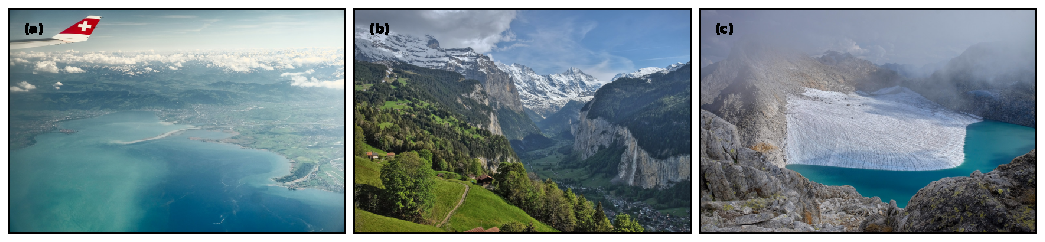
\includegraphics{alpero_landscape}}
      \caption{%
        Alpine glacial erosion landscape diversity.
        \textbf{(a)} Piedmont overdeepening of Lake Constance, ca.~10x50\,km.
        \textbf{(b)} Glacial trough of Lauterbrunnental, ca.~1x10\,km.
        \textbf{(c)} Mountain cirque of Chüebodengletscher, ca.~1x1\,km.}
      \label{fig:landscape}
    \end{figure*}

    \begin{figure*}
      \centerline{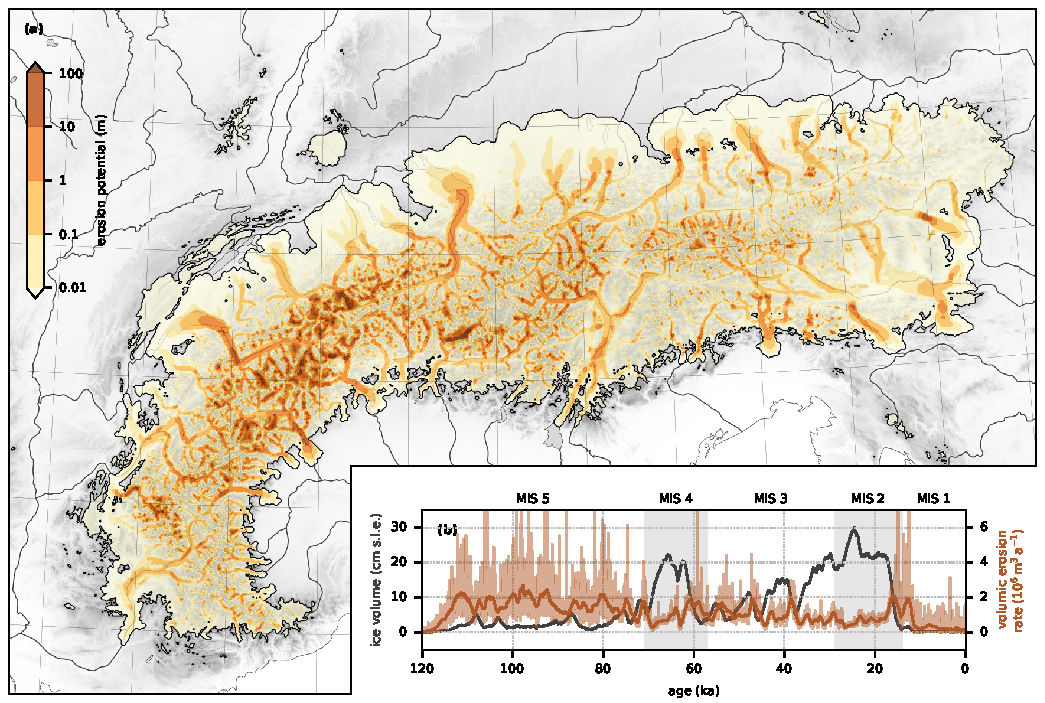
\includegraphics{alpero_cumulative}}
      \caption{%
        \textbf{(a)} Modelled cumulative (time-integrated) glacial erosion
          potential over the last glacial cycle.
        \textbf{(b)} Modelled total ice volume in centimetres of sea-level
          equivalent (cm~s.l.e., black), volumic (domain-integrated) erosion
          rate (light brown) and 100-a running mean (dark brown). Shaded gray
          areas indicate the timing for MIS~2 and~4
          \citep{Lisiecki.Raymo.2005}.} \label{fig:cumulative}
    \end{figure*}

    \begin{figure}
      \centerline{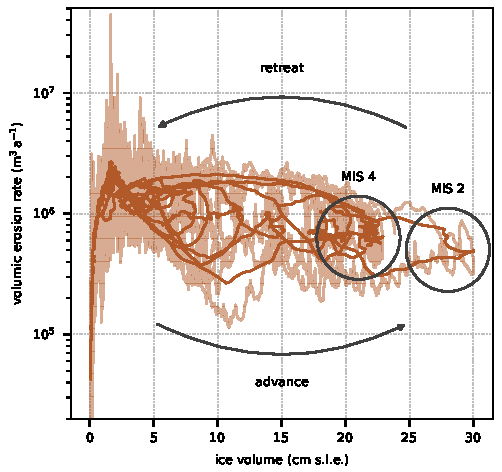
\includegraphics{alpero_evolution}}
      \caption{%
        Modelled volumic (domain-integrated) erosion rate (light brown) and 100-a
        running mean (dark brown) in relation to modelled total ice volume in
        centimetres of sea-level equivalent (black).}
      \label{fig:evolution}
    \end{figure}

    \begin{figure*}
      \centerline{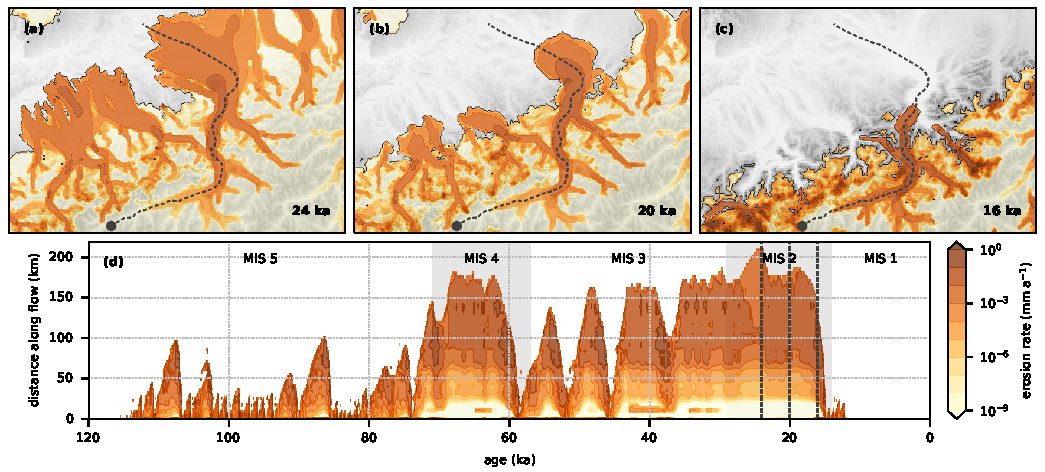
\includegraphics{alpero_transects}}
      \caption{%
        \textbf{(a, b, c)} Modelled instantaneous erosion rate of the Rhine
          Glacier for selected post-Last Glacial Maximum ages.
        \textbf{(d)} Interpolated instantaneous erosion rate along a Rhine
          Glacier transect for the entire last glacial cycle (upper panels
          dashed line).}
      \label{fig:transects}
    \end{figure*}

    \begin{figure*}
      \centerline{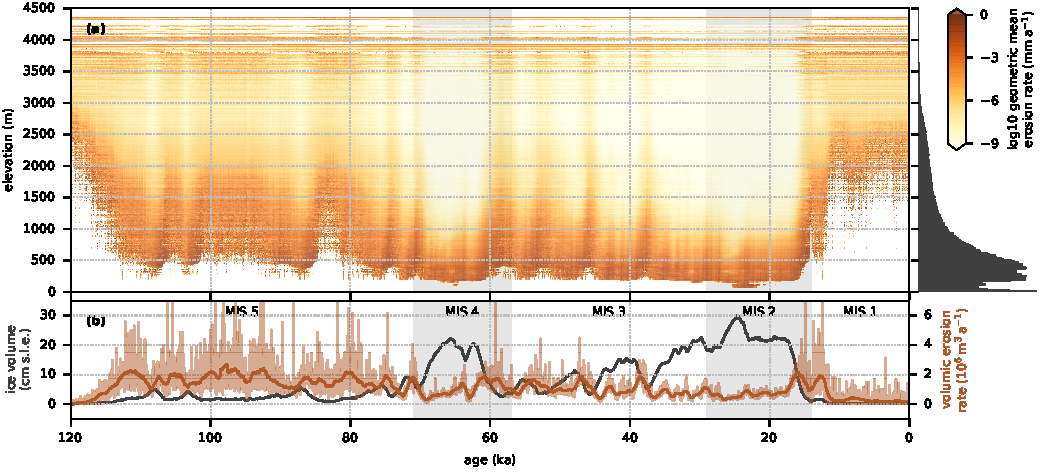
\includegraphics{alpero_hypsogram}}
      \caption{%
        \textbf{(a)} Modelled erosion rate ``hypsogram'', showing the geometric
          mean of (non-zero) modelled erosion rates in 10-m elevation bands
          across the entire model domain and its time evolution.
        \textbf{(b)} Same as Fig.~\ref{fig:cumulative}b.}
      \label{fig:hypsogram}
    \end{figure*}

    \begin{figure*}
      \centerline{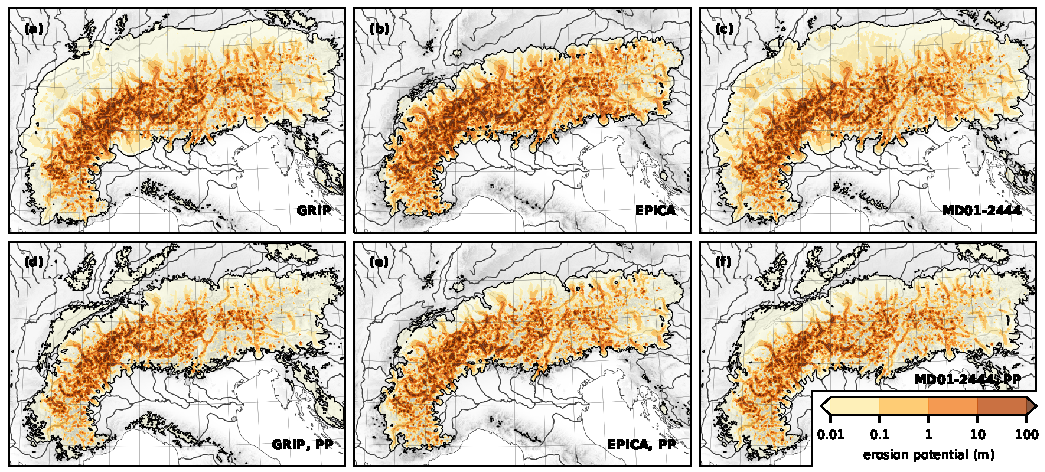
\includegraphics{alpero_sensitivity}}
      \caption{%
        Modelled cumulative glacial erosion potential over the last glacial
        cycle without \textbf{(a, b, c)} and with \textbf{(d, e, f)}
        paleo-precipitation corrections, and using three different
        palaeo-temperature histories \citep[see][]{Seguinot.etal.2018}.}
      \label{fig:sensitivity}
    \end{figure*}

    \begin{figure*}
      \centerline{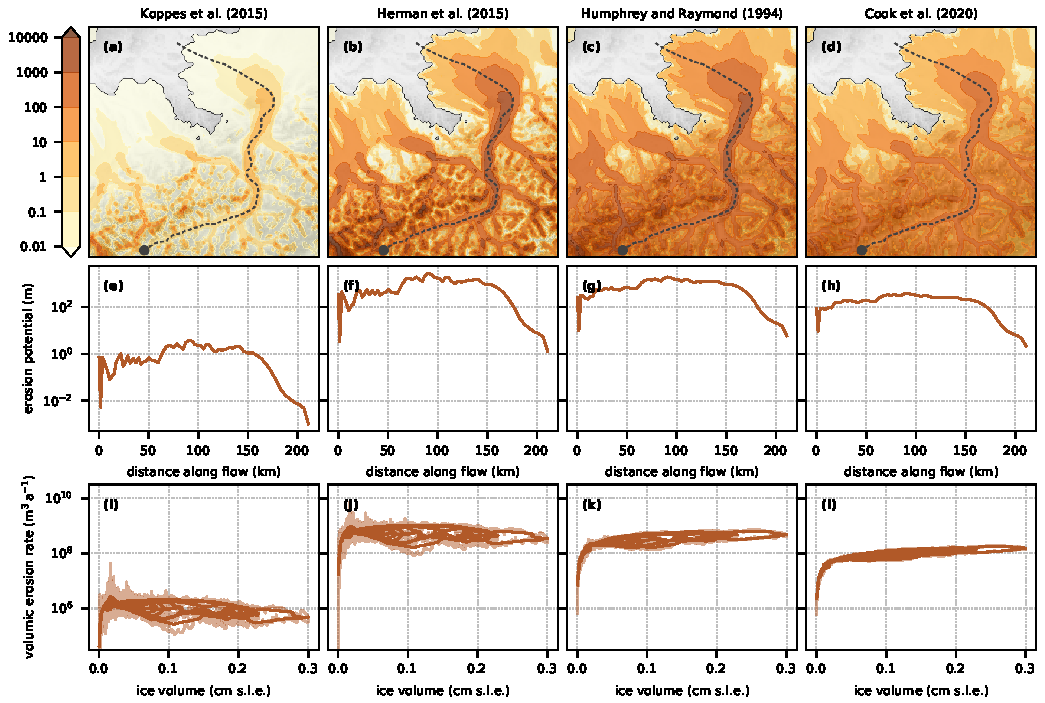
\includegraphics{alpero_powerlaws}}
      \caption{%
        Modelled cumulative (time-integrated) glacial erosion potential for
        three different erosion laws published by
        \textbf{(a)} \citet{Koppes.etal.2015},
          ${5.2 \times 10^{-8} u_\mathrm{b}^{2.34}}$ (same as
          Fig.~\ref{fig:cumulative}a but with a different colour scale),
        \textbf{(b)} \citet{Herman.etal.2015},
          ${2.7 \times 10^{-7} u_\mathrm{b}^{2.02}}$, and
        \textbf{(c)} \citet{Cook.etal.2020},
          ${1.665 \times 10^{-1} u_\mathrm{b}^{0.6459}}$.
        \textbf{(d)} Corresponding erosion power laws, and
        \textbf{(e)} modelled cumulative (time-integrated) glacial erosion
          potential along a Rhine Glacier transect (upper panels dashed line).}
      \label{fig:powerlaws}
    \end{figure*}

% ----------------------------------------------------------------------
% Tables
%\clearpage
% ----------------------------------------------------------------------


% ======================================================================
\end{document}
% ======================================================================
